% !TEX encoding = UTF-8
% !TEX TS-program = pdflatex
% !TEX root = ../tesi.tex

%**************************************************************
\chapter{Progettazione e codifica}
\label{cap:progettazione-codifica}
%**************************************************************

La seguente sezione ha lo scopo di illustrare la soluzione ideata dal laureando per il soddisfacimento dei requisiti concordati con il tutor aziendale descritti nel capitolo \ref{cap:descrizione-stage}. Nella prima sezione viene presentato l'applicativo con il dovuto corredo di immagini, mentre nel secondo viene descritta accuratamente l'architettura implementata.


\section{L'applicativo SyncRec}
\subsection{Struttura del progetto}
Come già accennato in precedenza, \textit{Angular} suggerisce di applicare una forte struttura modulare alle proprie \textit{web-application}, tale approccio è stato nella gran parte perseguito, con alcune eccezioni per determinati elementi condivisi fra più \textit{component}.

\begin{figure}[!h] 
	\centering 
	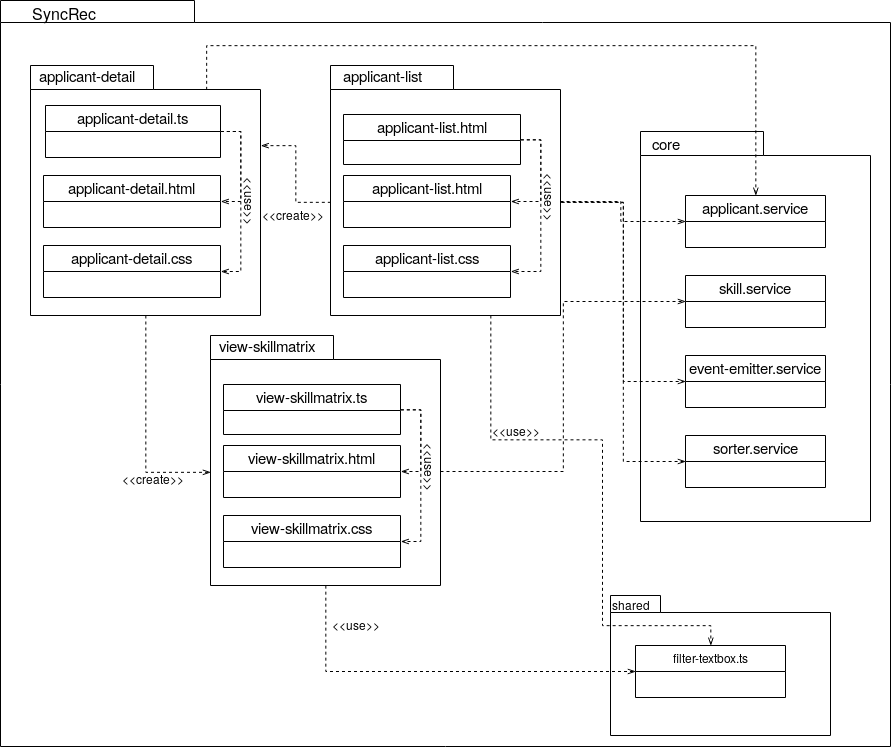
\includegraphics[width=1\columnwidth]{immagini/usecase/UML1} 
	\caption{Struttura dei component sviluppati per l'applicativo SyncRec}
	\label{figura:UML1}
\end{figure}

La figura \ref{figura:UML1} illustra la struttura dei component sviluppati per l'applicativo SyncRec, a scopo di sintesi sono state omesse alcune parti proprie del \textit{framework} di riferimento (come i moduli e gli \textit{asset}) o sviluppate da altri studenti nel corso del progetto.\\
I moduli \textit{applicant-list}, \textit{applicant-detail} e \textit{viewskillmatrix} rappresentano i componenti grafici dell'applicazione, il modulo \textit{shared} rappresenta l'insieme di \textit{component} condivisi nel \textit{namespace} globale e il modulo \textit{core} contiene i \textit{service}, i quali hanno il duplice scopo di recuperare i dati dal \textit{Back-end} e di fornire alcuni metodi di utilità necessari a svolgere determinate operazioni (come l'ordinamento o l'emissione di eventi verso \textit{components} padri).\\
La figura \ref{figura:UML2} illustra come il modulo \textit{service} si occupa di dialogare con il \textit{Back-end}scritto in \textit{Spring}.

\begin{figure}[!h] 
	\centering 
	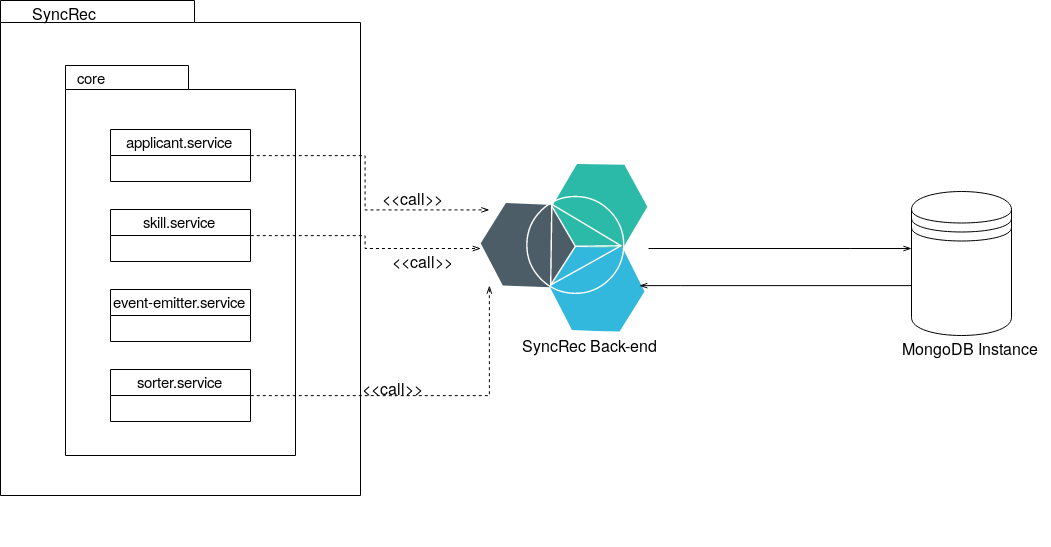
\includegraphics[width=1\columnwidth]{immagini/usecase/UML2} 
	\caption{Integrazione tra Front-end e Back-end}
	\label{figura:UML2}
\end{figure}

\subsection{Homepage}
\vspace{0.5em}
\begin{figure}[!h] 
	\centering 
	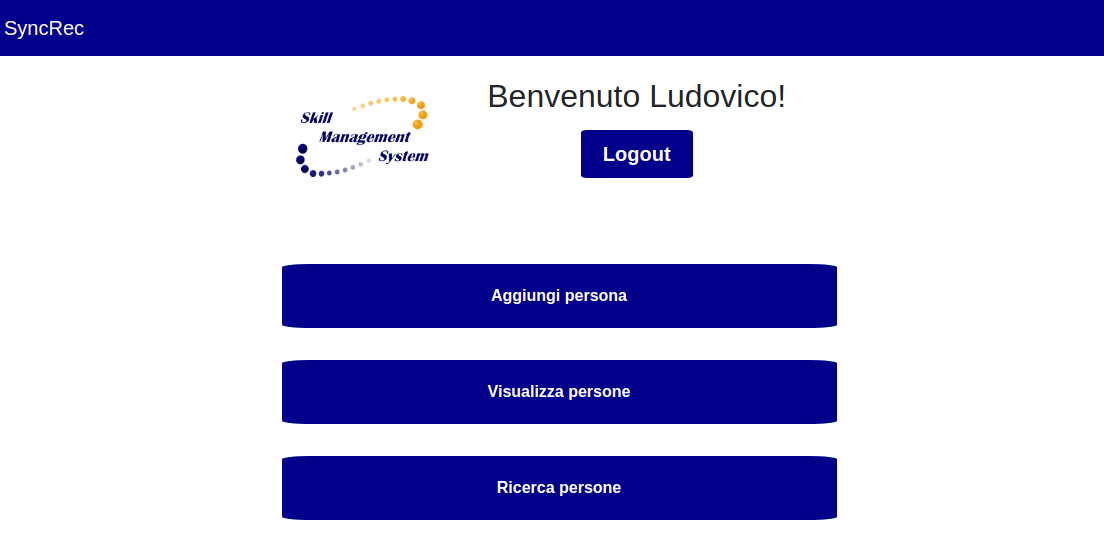
\includegraphics[width=1\columnwidth]{immagini/svil/homepage} 
	\caption{Schermata della homepage}
	\label{figura:homepage}
\end{figure}

\subsection{Maschera della visualizzazione degli\applicant}

\vspace{0.5em}
\begin{figure}[!h] 
	\centering 
	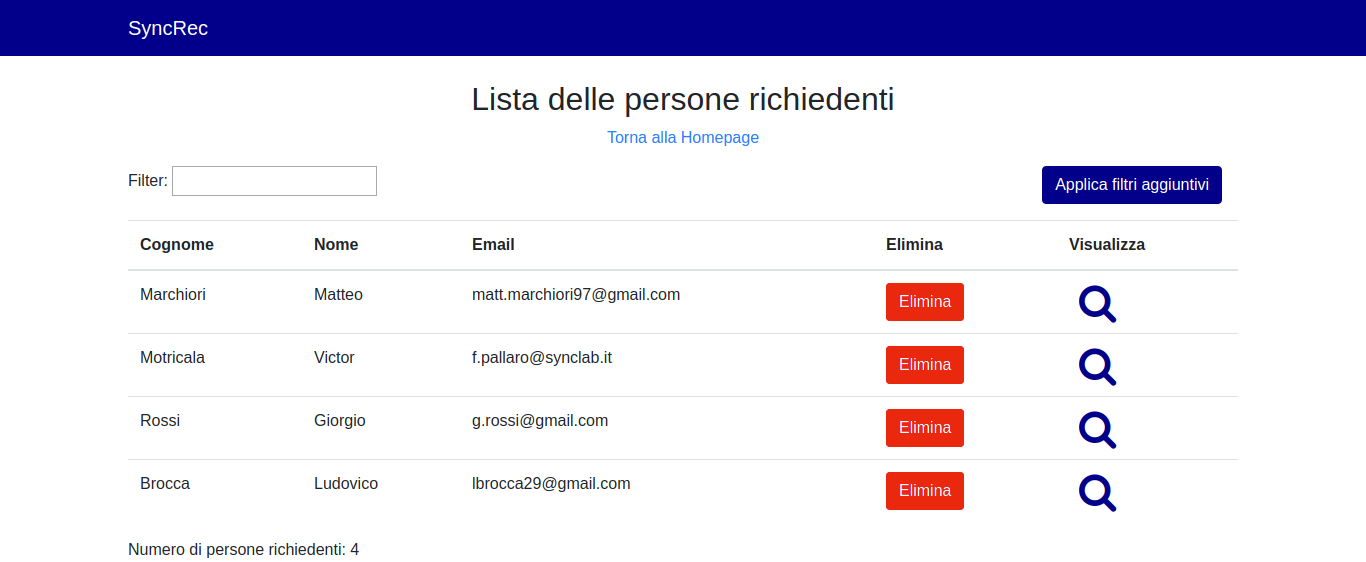
\includegraphics[width=1\columnwidth]{immagini/svil/lista} 
	\caption{Schermata della visualizzazione lista degli applicant}
	\label{figura:lista}
\end{figure}


\vspace{0.5em}
\begin{figure}[!h] 
	\centering 
	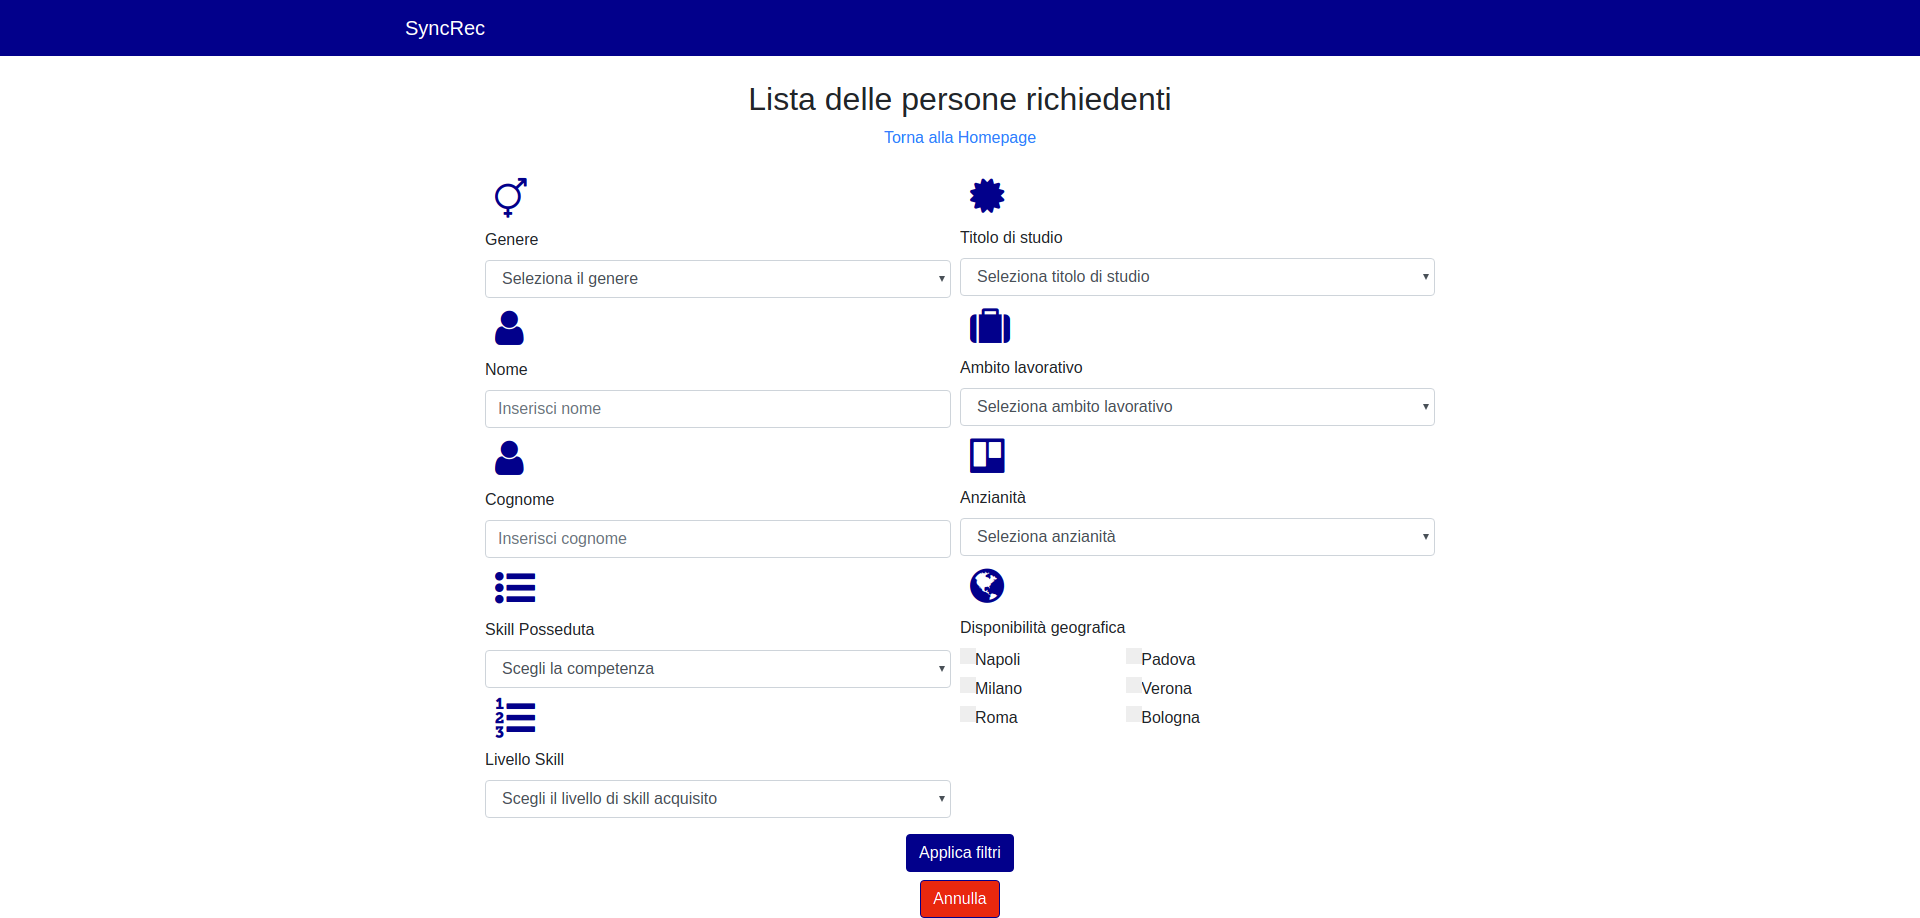
\includegraphics[width=1\columnwidth]{immagini/svil/filtri} 
	\caption{Schermata della selezione dei filtri da applicare alla lista degli applicant}
	\label{figura:filtri}
\end{figure}

\subsection{Maschera delle operazioni CRUD su un\applicant}
\vspace{0.5em}
\begin{figure}[!h] 
	\centering 
	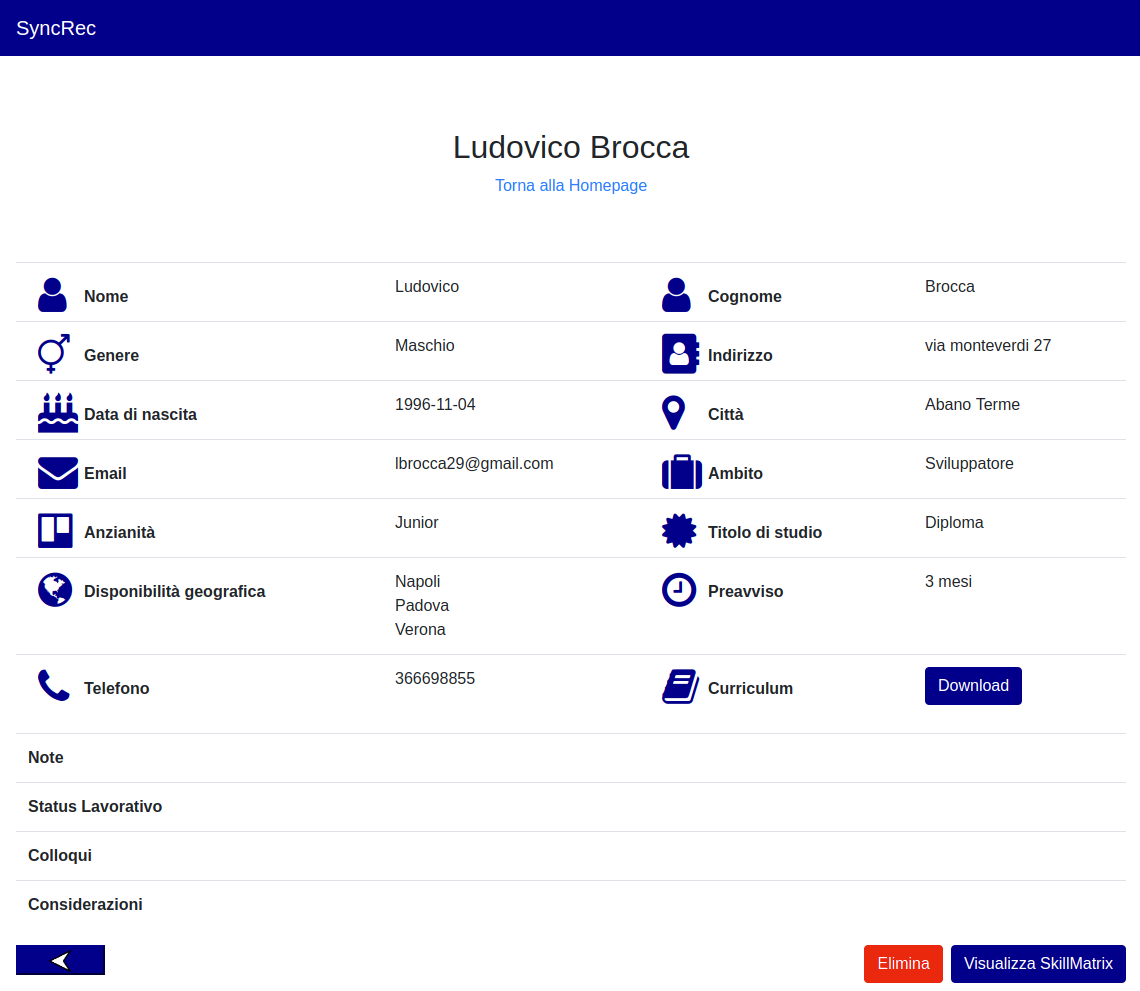
\includegraphics[width=1\columnwidth]{immagini/svil/applicant}
	\caption{Maschera CRUD del singolo applicant}
	\label{figura:applicant}
\end{figure}

\vspace{0.5em}
\begin{figure}[!h] 
	\centering 
	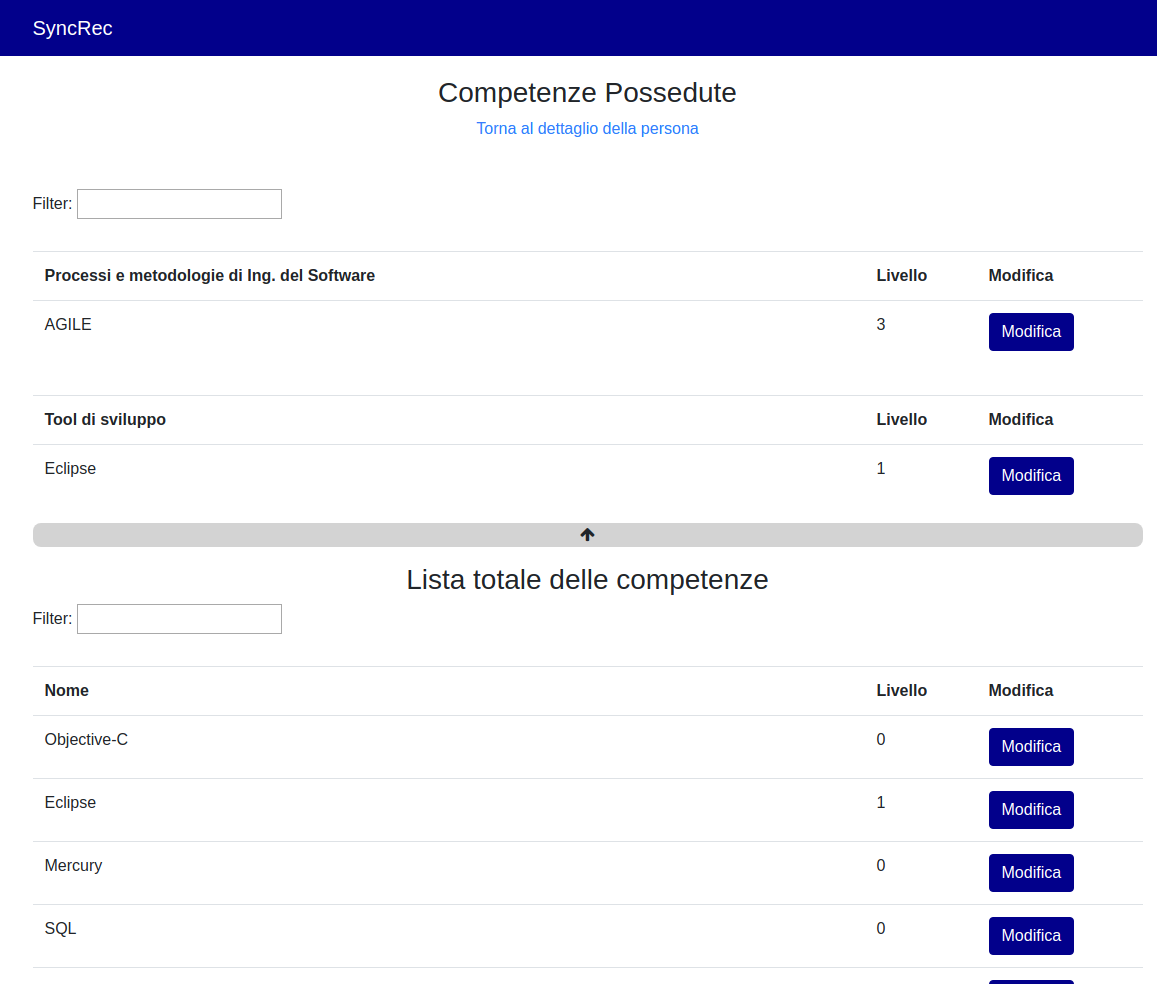
\includegraphics[width=1\columnwidth]{immagini/svil/skillmatrix} 
	\caption{Maschera CRUD dello skillmatrix}
	\label{figura:skillmatrix}
\end{figure}


\subsection{Sviluppo}
%Diagramma delle classi da fare qui%